\documentclass[12pt]{article}
\usepackage{amsmath}
\usepackage{graphicx,psfrag,bbm,epsf}
\usepackage{amssymb, amsmath, amsthm, color,enumerate,float,mathtools,graphicx,hyperref}
\usepackage{algorithm}
\usepackage[numbers]{natbib}
\usepackage{enumerate,multirow,booktabs}
\usepackage{url}
\usepackage{natbib}
\usepackage{url} % not crucial - just used below for the URL

%\pdfminorversion=4
% NOTE: To produce blinded version, replace "0" with "1" below.
\newcommand{\blind}{1}
\newtheorem{lem}{Lemma}
\newtheorem{thm}{Theorem}
\newtheorem*{thm*}{Theorem}
\newtheorem{pro}{Proposition}
\newtheorem{defn}{Definition}
\newtheorem{rmk}{Remark}
\newtheorem{cor}{Corollary}
\newcommand{\reals}{\mathbb{R}}
\newcommand{\naturals}{\mathbb{R}}
\newcommand{\vx}{\boldsymbol{x}}
\newcommand{\vt}{\boldsymbol{t}}
\newcommand{\vz}{\boldsymbol{z}}
\newcommand{\vy}{\boldsymbol{y}}
\newcommand{\dif}{{\rm d}}
\DeclareMathOperator{\sign}{sign}

\def\abs#1{\ensuremath{\left \lvert #1 \right \rvert}}


\newcommand{\FJH}[1]{{\color{blue}Fred: #1}}
\newcommand{\LK}[1]{{\color{green}Lulu: #1}} %choose your color
\newcommand{\YL}[1]{{\color{red}Yiou: #1}} %choose your color

\allowdisplaybreaks
\title{Inverse transformed points}
\author{ }
\date{November 2018}

\begin{document}

\maketitle

\section{A wrap up of meeting 11/20/2018:}
Structure and workflow of the paper:
\begin{enumerate}
    \item 
    Start with an example of performing inverse transformation method on low discrepancy sequence that produces large discrepancy with respect to normal measure.
    \begin{itemize}
        \item 
        Which discrepancy to use? $L_2$ discrepancy, centered $L_2$ or ....? \FJH{Use the centered $L_2$, but we may want to re-define it on a domain centered at the origin.}
        \item
        We decide to keep the kernel function fixed, but the discrepancy changes from
        $$[D(P;K)]^2 = \int_{\Omega\times\Omega} K(x,t)d[F_{\text{unif}}(x)-F_P(x)]d[F_{\text{unif}}(t)-F_P(t)]$$
        to
        $$[D(P;K)_{\text{normal}}]^2 = \int_{\Omega\times\Omega} K(x,t)d[\Phi(x)-F_P(x)]d[\Phi(t)-F_P(t)]$$
        \FJH{Here $F_P$ denotes the empirical distribution function of the design $P= \{x_i\}_{i=1}^N$.}
        \item
        The low discrepancy sequence that has small $[D(P;K)]^2$ may not retain small $[D(\Phi^{-1}(P));K)]^2_{\text{normal}}$ after applying inverse transformation.
    \end{itemize}
    \item
    Derive an analytical expression for $[D(P;K)_{\text{normal}}]^2$ so that we can evaluate it given a set of inverse transformed points. 
    \item
    Figure out a remedy for the issue. For instance take several low discrepancy sequences and evaluate $[D(P;K)_{\text{normal}}]^2$ of the inverse transformed sequences, then choose the one with the smallest $[D(P;K)_{\text{normal}}]^2$. Or, some optimization tools could be used to refine the inverse transformed points.
\end{enumerate}

\section{Intermediate Notes}
The reproducing kernel for centered $L_2$ discrepancy on $[0,1]^s$ is:
$$K(\vx,\vt) = \prod\limits_{j=1}^s\left[1+\frac{1}{2}|x_j-1/2|+\frac{1}{2}|t_j-1/2|-\frac{1}{2}|x_j-t_j|\right].$$
Transformed the kernel onto the region $[-1/2,1/2]^s$, we have:
\begin{align*}
    K(\vx,\vt) & = \prod\limits_{j=1}^s\left[1+\frac{1}{2}|x_j|+\frac{1}{2}|t_j|-\frac{1}{2}|x_j-t_j|\right] \\
\end{align*}
\FJH{Let $P = \{x_i\}_{i=1}^N$ be a possible design.}  Then, the discrepancy of the design $P$ w.r.t.\ the standard multivariate normal probability distribution $\Phi$, which has domain $\Omega = (-\infty,\infty)^s$ is
\begin{eqnarray*}
&&[D(P)]^2\\
&=& \int_{\Omega\times \Omega} K(\vx,\vt)\dif \Phi(\vx)\dif \Phi(\vt)-\frac{2}{N}\sum_{n=1}^N \int_{\Omega}K(\vx,\vx_n)\dif \Phi(\vx)+\frac{1}{N^2}\sum_{n,m=1}^N K(\vx_n,\vx_m)\\
\end{eqnarray*}
\textcolor{red}{From Lulu: by a design $P$, do you mean a sample of $\{x_i\}_{i=1}^N$ that is sampled from $P$? This part is not very clear to me.}

\begin{enumerate}
    \item ($s=1$)
    \FJH{Note that this reproducing kernel corresponds to the inner product
    \begin{equation}
        \langle f,g \rangle = f(0) g(0)  + \int_{-\infty}^\infty f'(x) g'(x) \, \dif x
    \end{equation}
    To demonstrate this, note that
    \begin{align*}
        K(0,t) &= 1, \\
        \frac{\partial K(x,t)}{\partial x} &= \frac 12 \left[\sign(x) - \sign(x - t) \right] \\
        & = \begin{cases} 0, & -\infty < x < \min(0,t), \\
        \sign(t), & \min(0,t) < x < \max(0,t), \\
        0, & \max(0,t) < x < \infty,
        \end{cases}
        \\
        \intertext{so $\langle K(\cdot,t), K(\cdot,t) \rangle < \infty $, and}
        \langle f, K(\cdot,t) \rangle &= f(0) K(0,t) + \int_{-\infty}^\infty f'(x) \frac{\partial K(x,t)}{\partial x} \, \dif x \\
        & = f(0) + \sign(t) \int_{\min(0,t)}^{\max(0,t)} f'(x)  \, \dif x \\    
        & = f(0) + \sign(t) [f(\max(0,t)) - f(\min(0,t))] \\    
        & = f(t)
        \end{align*}
        
        To compute the discrepancy, we first integrate the kernel once:
       \begin{align*}
  \MoveEqLeft{\int_{-\infty}^\infty K(x,t) \, \dif \Phi(x)}\\
    & =  \int_{-\infty}^{\infty} \left(1+\frac{1}{2}|x|+\frac{1}{2}|t|-\frac{1}{2}|x-t|\right)\phi(x) \, \dif x\\
    &= 1+ \frac{1}{\sqrt{2\pi}} + \frac{1}{2}|t|-\frac{1}{2}\left[\int_{-\infty}^{t}(t-x)\phi(x) \, \dif x+\int_{t}^{\infty} (x-t)\phi(x) \, \dif x\right]\\
    &= 1+ \frac{1}{\sqrt{2\pi}} + \frac{1}{2}|t| - t [\Phi(t)-1/2] - \phi(t) .
    \end{align*}
    Then we integrate again:
       \begin{align*}
  \MoveEqLeft{\int_{-\infty}^\infty \int_{-\infty}^\infty K(x,t) \, \dif \Phi(x) \dif \Phi(t)}\\
    & =  \int_{-\infty}^{\infty} \left( 1+ \frac{1}{\sqrt{2\pi}} + \frac{1}{2}|t| - t [\Phi(t)-1/2] +  \phi(t) \right)\phi(t) \, \dif t\\
    &= 1+ \sqrt{\frac{2}{\pi}} + \int_{-\infty}^{\infty} \{ - t \Phi(t)\phi(t)  +  [\phi(t)]^2 \} \, \dif t\\
    &= 1+\sqrt{\frac{2}{\pi}}-\frac{1}{\sqrt{4\pi}}+\int_{-\infty}^{\infty}\frac{1}{2\pi}e^{-t^2}\dif t\\
    &= 1+\sqrt{\frac{2}{\pi}}-\frac{1}{\sqrt{4\pi}}+\frac{\frac{1}{\sqrt{2}}}{\sqrt{2\pi}}\int_{-\infty}^{\infty}\frac{1}{\sqrt{2\pi}\left(\frac{1}{\sqrt{2}}\right)}e^{-\frac{t^2}{2\left(\frac{1}{\sqrt{2}}\right)^2}}\dif t\\
    &=1+\sqrt{\frac{2}{\pi}}
    \end{align*}
  
  $\int_{-\infty}^{\infty} t\Phi(t)\phi(t)\dif t = \frac{1}{\sqrt{4\pi}}$ comes from the link: \href{https://en.wikipedia.org/wiki/List_of_integrals_of_Gaussian_functions}{List of integrals of Gaussian functions.}
    }
    
    
    \begin{eqnarray*}
  &&  \int_{\Omega}K(x,x_n)\dif \Phi(x)\\
    &=& \int_{-\infty}^{\infty} \left(1+\frac{1}{2}|x|+\frac{1}{2}|x_n|-\frac{1}{2}|x-x_n|\right)\phi(x)\dif x\\
    &=& 1+\frac{1}{2}\sqrt{\frac{2}{\pi}}+\frac{1}{2}|x_n|-\frac{1}{2}\left[\int_{-\infty}^{x_n}(x_n-x)\phi(x)\dif x+\int_{x_n}^{\infty} (x-x_n)\phi(x)\dif x\right]\\
    &=& 1+\sqrt{\frac{1}{2\pi}}+\frac{1}{2}|x_n|-\frac{1}{2}\left[\int_{-\infty}^{x_n}(x_n-x)\phi(x)\dif x+\int_{x_n}^{\infty} (x-x_n)\phi(x)\dif x\right]\\
    &=& 1+\sqrt{\frac{1}{2\pi}}+\frac{1}{2}|x_n|-\frac{1}{2}\left[2x_n\Phi(x_n)-x_n-2\int_{-\infty}^{x_n}x\phi(x)\dif x\right]\\
    &=& 1+\sqrt{\frac{1}{2\pi}}+\max(x_n,0)-x_n\Phi(x_n)-\frac{ e^{-x_n^2/2}}{\sqrt{2\pi}}
    \end{eqnarray*}
    Thus, the discrepancy becomes
    \begin{eqnarray*}
   && [D(P)]^2\\
    &= &1+\sqrt{\frac{2}{\pi}}-\frac{2}{N}\sum_{n=1}^N \left[1+\sqrt{\frac{1}{2\pi}}+\max(x_n,0)-x_n\Phi(x_n)-\frac{ e^{-x_n^2/2}}{\sqrt{2\pi}}\right]\\
    &&+\frac{1}{N^2}\sum_{n,m=1}^N \left[1+\frac{1}{2}|x_n|+\frac{1}{2}|x_m|-\frac{1}{2}|x_n-x_m|\right]\\
     &= &-\frac{2}{N}\sum_{n=1}^N \left[\max(x_n,0)-x_n\Phi(x_n)-\frac{ e^{-x_n^2/2}}{\sqrt{2\pi}}\right]+\frac{1}{N^2}\sum_{n,m=1}^N \left[\frac{1}{2}|x_n|+\frac{1}{2}|x_m|-\frac{1}{2}|x_n-x_m|\right]\\
     &=& -\frac{2}{N}\sum_{n=1}^N \left[\max(x_n,0)-x_n\Phi(x_n)-\phi(x_n)\right]+\frac{1}{N}\sum_{n=1}^N|x_n|-\frac{1}{2N^2}\sum_{n,m=1}^N|x_n-x_m|\\ &&(\text{the last expression is for coding purpose only})
    \end{eqnarray*}
    
   \item ($s>1$)
   \begin{enumerate}
       \item 
       i.i.d. standard Normal random variables, the joint pdf 
       $$\Phi(\vx) = \prod\limits_{j=1}^s\Phi_0(x_j) = \prod\limits_{j=1}^s \frac{1}{\sqrt{2\pi}}e^{-x_j^2/2}.$$
       Thus, 
       $$\int_{\reals^s\times \reals^s} K(\vx,\vt)\dif\Phi(\vx)\dif\Phi(\vt) = \left(1+\sqrt{\frac{2}{\pi}}\right)^s,$$
       $$\int_{\reals^d}K(\vx,\vx_n)\dif\Phi(\vx) = \prod\limits_{j=1}^s\left[ 1+\frac{1}{\sqrt{2\pi}}+\frac{1}{2}|x_j|-x_j[\Phi_0(x_j)-1/2]-\phi(x_j)\right].$$
       Thus, the discrepancy becomes:
       \begin{eqnarray*}
 &&[D(P)]^2\\
  &=& \left(1+\sqrt{\frac{2}{\pi}}\right)^s - \frac{2}{N}\sum\limits_{\vx\in P} \prod\limits_{j=1}^s\left[ 1+\frac{1}{\sqrt{2\pi}}+\frac{1}{2}|x_j|-x_j[\Phi_0(x_j)-1/2]-\phi(x_j)\right]\\
  &&+\frac{1}{N^2}\sum_{\vx,\vx'\in P}\prod_{j=1}^s \left[1+\frac{1}{2}|x_j|+\frac{1}{2}|x'_j|-\frac{1}{2}|x_j-x'_j|\right]
\end{eqnarray*}       
   \end{enumerate}
   
   
\end{enumerate}

\section{Notes on Issues (1/17/2019)}
$N$ is the sample size and I move the largest point in Sobol sequence to the boundary $1-10^{-15}$. $x$ is the Sobol sequence, $y$ is $x$ with largest point moved to $1-10^{-15}$, and $z$ is the uniform random numbers generated by Matlab. Then, I compare the normal discrepancies after inverse transformation. Here ere are some numerical results I have:
\begin{enumerate}
\item
Overall, the normal discrepancy of transformed $y$ is not very different from that of transformed $x$. 
    \item 
    In one of my simulations, the discrepancy of $y$ is smaller than discrepancy of $z$, but the after inverse transformation, the normal discrepancy of transformed $y$ becomes larger than the normal discrepancy of transformed $z$.
    \item
    I found that the normal discrepancy doesn't change much as the sample size $N$ changes, e.g., when $N=10$, the normal discrepancy of normal random numbers generated by Matlab is 0.6164; when $N=100$, it becomes 0.5765; when $N=1000$, it becomes 0.5647; when $N=10000$, it becomes 0.5642. 
    \item
    What's more, even when we calculate the normal discrepancy of a Sobol sequence (which is uniformly distributed on [0,1]. This sequence should have large normal discrepancy as it doesn't even contain any negative number.), with $N=100$, the normal discrepancy is 0.7571 which is not as large as I expected.
    \item
    This normal discrepancy can be large, e.g. the normal discrepancy of a sample with two points -10 and 10 is 5. However, the normal discrepancy of `randn(100,1)' is about 0.5694, and if we change one point to 10 (10 standard deviation above the mean), the normal discrepancy only changes to about 0.5699. If we use a smaller sample, e.g., the normal discrepancy of `randn(10,1)' is about 0.5878,   and if we change one point to 10, the normal discrepancy changes to about 0.6992. So, I think when the sample size is large, the normal discrepancy is not sensitive to the change of one point. 
\end{enumerate}
What Lulu and I suspect is that the problem lies in the kernel we choose. This normal discrepancy doesn't really distinguish the samples well. 

Also, I think the discrepancy may become more different if we have a larger dimension and the sample is more sparse. But, note that for 1-d situation, the centered $L_2$ uniform discrepancy still distinguishes the samples very well even when the sample size is large.

\section{A Motivation Example}
Consider dimension of input factor $s=10$, and sample size $N=2^10$. Move the the point that is nearest to the origin in Sobol sequence $\vx$ to $(10^{-15},...,10^{-15})$, and the new sequence is denoted by $\vy$. $\vz$ is a sample of uniform random points of size $N$. The following table includes the uniform discrepancy and the normal discrepancy after inverse distribution transformation.
% Table generated by Excel2LaTeX from sheet 'Sheet1'
\begin{table}[H]
  \centering
    \begin{tabular}{ccc}
     Sample     & Uniform Discrepancy & Normal Discrepancy \\
    \hline
    $\vx$     & 0.0285 & 18.5713 \\
   $\vy$     & 0.0292 & 58.8191 \\
    $\vz$     & 0.0802 & 18.5748 \\
    \end{tabular}%
\end{table}%

\section{Coordinate Exchange}
When we remove one point $\vx^i = [x^i_{1},x^i_{2},...,x^i_{s}]$ from the sample, the change in the squared discrepancy is:
\begin{eqnarray*}
&&D^2(P\backslash \vx^i)-D^2(P)\\
&=& -\frac{2}{N-1}\sum\limits_{\vx\in P\backslash \vx^i} \prod\limits_{j=1}^s\left[ 1+\frac{1}{\sqrt{2\pi}}+\frac{1}{2}|x_j|-x_j[\Phi_0(x_j)-1/2]-\phi(x_j)\right]\\
  &&+\frac{1}{(N-1)^2}\sum_{\vx,\vx'\in P\backslash\vx^i}\prod_{j=1}^s \left[1+\frac{1}{2}|x_j|+\frac{1}{2}|x'_j|-\frac{1}{2}|x_j-x'_j|\right]\\
  &&+\frac{2}{N}\sum\limits_{\vx\in P} \prod\limits_{j=1}^s\left[ 1+\frac{1}{\sqrt{2\pi}}+\frac{1}{2}|x_j|-x_j[\Phi_0(x_j)-1/2]-\phi(x_j)\right]\\
  &&-\frac{1}{N^2}\sum_{\vx,\vx'\in P}\prod_{j=1}^s \left[1+\frac{1}{2}|x_j|+\frac{1}{2}|x'_j|-\frac{1}{2}|x_j-x'_j|\right]\\
  &=& -\frac{2}{N-1}\sum\limits_{\vx\in P} \prod\limits_{j=1}^s\left[ 1+\frac{1}{\sqrt{2\pi}}+\frac{1}{2}|x_j|-x_j[\Phi_0(x_j)-1/2]-\phi(x_j)\right]\\
  &&+\frac{1}{(N-1)^2}\sum_{\vx,\vx'\in P}\prod_{j=1}^s \left[1+\frac{1}{2}|x_j|+\frac{1}{2}|x'_j|-\frac{1}{2}|x_j-x'_j|\right]\\
  &&+\frac{2}{N-1}\prod\limits_{j=1}^s\left[ 1+\frac{1}{\sqrt{2\pi}}+\frac{1}{2}|x^i_{j}|-x_j[\Phi_0(x^i_{j})-1/2]-\phi(x^i_{j})\right]\\
  && - \frac{1}{(N-1)^2}\left(2\sum_{\vx'\in P\backslash \vx^i}\prod_{j=1}^s \left[1+\frac{1}{2}|x^i_{j}|+\frac{1}{2}|x'_j|-\frac{1}{2}|x^i_{j}-x'_j|\right]+\prod_{j=1}^s\left[1+|x^i_{j}|\right]\right)\\
  &&+\frac{2}{N}\sum\limits_{\vx\in P} \prod\limits_{j=1}^s\left[ 1+\frac{1}{\sqrt{2\pi}}+\frac{1}{2}|x_j|-x_j[\Phi_0(x_j)-1/2]-\phi(x_j)\right]\\
  &&-\frac{1}{N^2}\sum_{\vx,\vx'\in P}\prod_{j=1}^s \left[1+\frac{1}{2}|x_j|+\frac{1}{2}|x'_j|-\frac{1}{2}|x_j-x'_j|\right]\\
  &=&  -\frac{2}{N(N-1)}\sum\limits_{\vx\in P} \prod\limits_{j=1}^s\left[ 1+\frac{1}{\sqrt{2\pi}}+\frac{1}{2}|x_j|-x_j[\Phi_0(x_j)-1/2]-\phi(x_j)\right]\\
  && +\frac{2N-1}{N^2(N-1)^2} \sum_{\vx,\vx'\in P}\prod_{j=1}^s \left[1+\frac{1}{2}|x_j|+\frac{1}{2}|x'_j|-\frac{1}{2}|x_j-x'_j|\right]\\
&&+\frac{2}{N-1}\prod\limits_{j=1}^s\left[ 1+\frac{1}{\sqrt{2\pi}}+\frac{1}{2}|x^i_{j}|-x_j[\Phi_0(x^i_{j})-1/2]-\phi(x^i_{j})\right]\\
  && - \frac{1}{(N-1)^2}\left(2\sum_{\vx'\in P\backslash\vx^i}\prod_{j=1}^s \left[1+\frac{1}{2}|x^i_{j}|+\frac{1}{2}|x'_j|-\frac{1}{2}|x^i_{j}-x'_j|\right]+\prod_{j=1}^s\left[1+|x^i_{j}|\right]\right)\\
\end{eqnarray*}

Define the row deletion function when we remove a point $\vx_i$ as
\begin{eqnarray}\label{eq:rowdelection}
d_r(\vx^i) &=& -2\prod\limits_{j=1}^s\left[ 1+\frac{1}{\sqrt{2\pi}}+\frac{1}{2}|x^i_{j}|-x_j[\Phi_0(x^i_{j})-1/2]-\phi(x^i_{j})\right]\\ \nonumber
  && + \frac{1}{N-1}\left(2\sum_{\vx'\in P}\prod_{j=1}^s \left[1+\frac{1}{2}|x^i_{j}|+\frac{1}{2}|x'_j|-\frac{1}{2}|x^i_{j}-x'_j|\right]-\prod_{j=1}^s\left[1+|x^i_{j}|\right]\right)
\end{eqnarray}
(Note: The elements of the first and third tensor products are stored in the $i$th row of the sample matrix. The elements in the sum are stored in the $i$th column of the distance matrix $D$.)

Sample the index $i^*$ from $\{1,...,N\}$ with probability $
\frac{d_r(\vx^i)}{\sum\limits_{j=1}^Nd_r(\vx^j)}$.

The column deletion function for the $j$th column ($X_k$) of the sample is:
\begin{eqnarray}
d_c(X_k) &=& D^2(P)-D^2(P') \nonumber\\
&=& -2\sum_{\vx\in P}\prod\limits_{\substack{j=1\\j\neq k}}^s\left[ 1+\frac{1}{\sqrt{2\pi}}+\frac{1}{2}|x_{j}|-x_j[\Phi_0(x_{j})-1/2]-\phi(x_{j})\right]\nonumber\\ 
&&\left(\frac{1}{\sqrt{2\pi}}+\frac{1}{2}|x_{k}|-x_k[\Phi_0(x_{k})-1/2]-\phi(x_{k})\right)\nonumber\\
&&+\frac{1}{N}\sum_{\vx,\vx'\in P}\prod_{\substack{j=1\\j\neq k}}^s \left[1+\frac{1}{2}|x_j|+\frac{1}{2}|x'_j|-\frac{1}{2}|x_j-x'_j|\right]\left(\frac{1}{2}|x_k|+\frac{1}{2}|x_k'|-\frac{1}{2}|x_k-x_k'|\right)
\end{eqnarray}

(Note that the terms in the tensor product are already stored in the distance matrix and are only calculated once.)

The delta function for exchanging the $i$th point $\vx^i$ with an alternative is (sample changes from $P$ to  $P' = P\backslash\vx^i\cup \vx$):
\begin{eqnarray*}
&&\Delta(\vx^i,\vx)\\
&=& [D(P')]^2-[D(P)]^2\\
&=& \frac{2}{N}\left(\prod\limits_{j=1}^s\left[ 1+\frac{1}{\sqrt{2\pi}}+\frac{1}{2}|x^i_{j}|-x_j[\Phi_0(x^i_{j})-1/2]-\phi(x^i_{j})\right]\right.\\
&&\left.-\prod\limits_{j=1}^s\left[ 1+\frac{1}{\sqrt{2\pi}}+\frac{1}{2}|x_{j}|-x_j[\Phi_0(x_{j})-1/2]-\phi(x_{j})\right]\right)\\
&&+\frac{1}{N^2}\left(2\sum_{\vz\in P'}\prod_{j=1}^s \left[1+\frac{1}{2}|x_{j}|+\frac{1}{2}|z_j|-\frac{1}{2}|x_{j}-z_j|\right]-\prod_{j=1}^s\left[1+|x_{j}|\right]\right.\\
&& - \left.2\sum_{\vz\in P}\prod_{j=1}^s \left[1+\frac{1}{2}|x^i_{j}|+\frac{1}{2}|z_j|-\frac{1}{2}|x^i_{j}-z_j|\right]+\prod_{j=1}^s\left[1+|x^i_{j}|\right]\right)
\end{eqnarray*}

If only one coordinate $j^*$ of the point $\vx^{i^*}$ is allowed to change, the delta function for exchanging $x_{{i^*},{j^*}}$ with $x\in \mathbb{R}$ is:
\begin{eqnarray*}
&&\Delta(x_{{i^*},{j^*}}, x)\\
&=& \frac{2}{N}\prod\limits_{\substack{j=1,\\j\neq j^*}}^s\left[ 1+\frac{1}{\sqrt{2\pi}}+\frac{1}{2}|x^{i^*}_{j}|-x_j[\Phi_0(x^{i^*}_{j})-1/2]-\phi(x^{i^*}_{j})\right]\\
&&\left[\frac{1}{2}\left(|x|-|x_{{i^*},{j^*}}|+x-x_{{i^*},{j^*}}\right)-x\Phi_0(x)+x_{{i^*},{j^*}}\Phi_0(x_{{i^*},{j^*}})-\phi(x)+\phi(x_{{i^*},{j^*}})\right]\\
&&+\frac{1}{N^2}\left(\sum_{\vz\in P\backslash \vx^{i^*}}\prod_{\substack{j=1,\\j\neq j^*}}^s\left[1+\frac{1}{2}|x_{j}|+\frac{1}{2}|z_j|-\frac{1}{2}|x_{j}-z_j|\right]\left[|x|-|x-z_{j^*}|-|x_{i^*,j^*}|+|x_{i^*,j^*}-z_{j^*}|\right]\right.\\
&&+\left.\prod_{\substack{j=1,\\j\neq j^*}}^s[1+|x_{i^*,j}|](|x|-|x_{i^*,j^*}|)\right)
\end{eqnarray*}
After choosing a particular dimension of a particular point, it becomes a univariate optimization problem of minimizing the delta function $\Delta(x_{{i^*},{j^*}}, x)$.
\newpage
\section{Numerical Results}
The proposed algorithm works as follows:
\begin{enumerate}
    \item 
    Generate a Sobol sequence of size $N$ with dimension $d$.
    \item
    Use inverse distribution transformation to transform uniform random numbers to generate normal random numbers.
    \item
    Use coordinate exchange algorithm to minimize the normal discrepancy.
\end{enumerate}

\underline{Examples}:
\begin{enumerate}
    \item 
    ($d=5, n=50$)
\begin{figure}[H]
\centering
{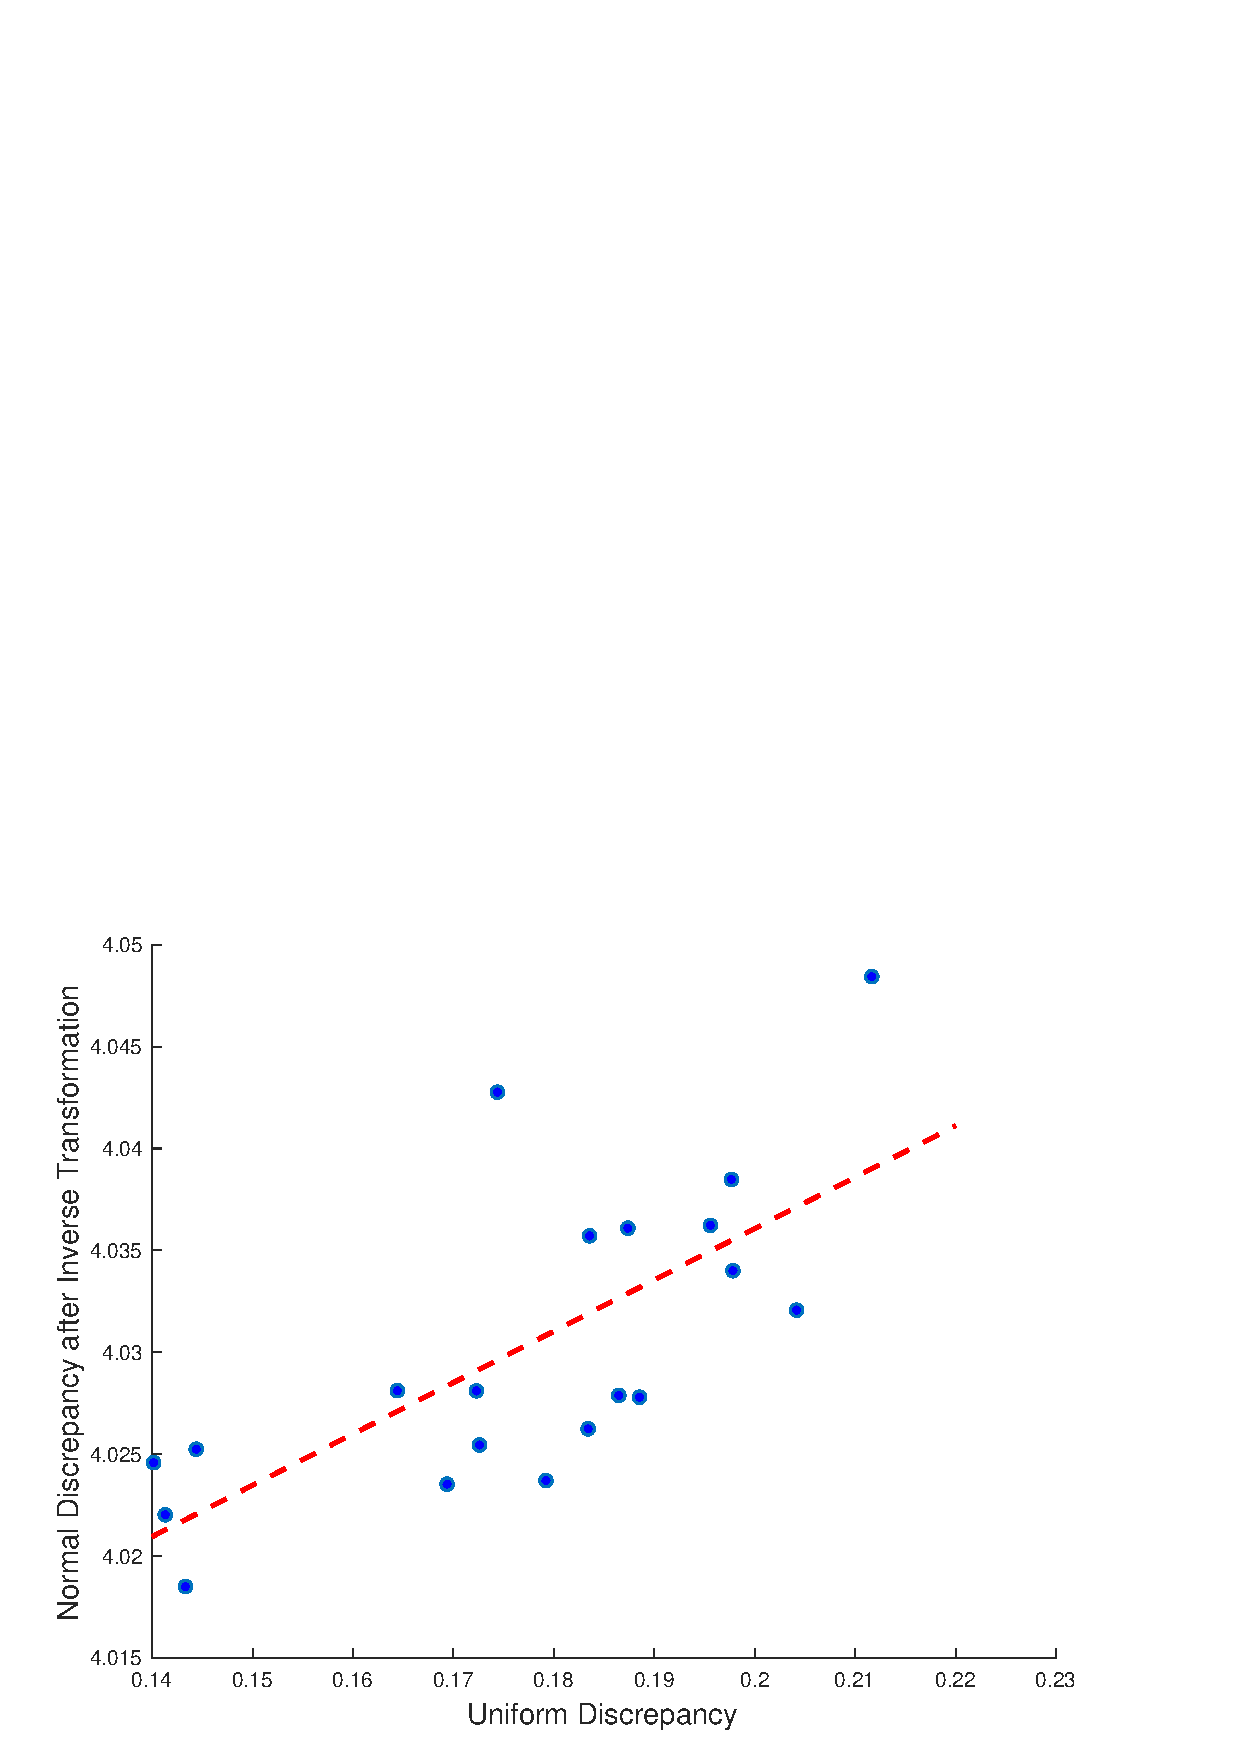
\includegraphics[width=8cm]{d5n50.pdf}}
\end{figure}
\begin{figure}[H]
\centering
{\includegraphics[width=8cm]{d5n50_invsobol.pdf}}
\end{figure}

    
\end{enumerate}

\end{document}
